% Options for packages loaded elsewhere
\PassOptionsToPackage{unicode}{hyperref}
\PassOptionsToPackage{hyphens}{url}
%


\PassOptionsToPackage{table}{xcolor}

\documentclass[
  10pt,
  letterpaper,
]{article}

\usepackage{amsmath,amssymb}
\usepackage{iftex}
\ifPDFTeX
  \usepackage[T1]{fontenc}
  \usepackage[utf8]{inputenc}
  \usepackage{textcomp} % provide euro and other symbols
\else % if luatex or xetex
  \usepackage{unicode-math}
  \defaultfontfeatures{Scale=MatchLowercase}
  \defaultfontfeatures[\rmfamily]{Ligatures=TeX,Scale=1}
\fi
\usepackage{lmodern}
\ifPDFTeX\else  
    % xetex/luatex font selection
\fi
% Use upquote if available, for straight quotes in verbatim environments
\IfFileExists{upquote.sty}{\usepackage{upquote}}{}
\IfFileExists{microtype.sty}{% use microtype if available
  \usepackage[]{microtype}
  \UseMicrotypeSet[protrusion]{basicmath} % disable protrusion for tt fonts
}{}
\makeatletter
\@ifundefined{KOMAClassName}{% if non-KOMA class
  \IfFileExists{parskip.sty}{%
    \usepackage{parskip}
  }{% else
    \setlength{\parindent}{0pt}
    \setlength{\parskip}{6pt plus 2pt minus 1pt}}
}{% if KOMA class
  \KOMAoptions{parskip=half}}
\makeatother
\usepackage{xcolor}
\usepackage[top=0.85in,left=2.75in,footskip=0.75in]{geometry}
\setlength{\emergencystretch}{3em} % prevent overfull lines
\setcounter{secnumdepth}{-\maxdimen} % remove section numbering


\providecommand{\tightlist}{%
  \setlength{\itemsep}{0pt}\setlength{\parskip}{0pt}}\usepackage{longtable,booktabs,array}
\usepackage{calc} % for calculating minipage widths
% Correct order of tables after \paragraph or \subparagraph
\usepackage{etoolbox}
\makeatletter
\patchcmd\longtable{\par}{\if@noskipsec\mbox{}\fi\par}{}{}
\makeatother
% Allow footnotes in longtable head/foot
\IfFileExists{footnotehyper.sty}{\usepackage{footnotehyper}}{\usepackage{footnote}}
\makesavenoteenv{longtable}
\usepackage{graphicx}
\makeatletter
\def\maxwidth{\ifdim\Gin@nat@width>\linewidth\linewidth\else\Gin@nat@width\fi}
\def\maxheight{\ifdim\Gin@nat@height>\textheight\textheight\else\Gin@nat@height\fi}
\makeatother
% Scale images if necessary, so that they will not overflow the page
% margins by default, and it is still possible to overwrite the defaults
% using explicit options in \includegraphics[width, height, ...]{}
\setkeys{Gin}{width=\maxwidth,height=\maxheight,keepaspectratio}
% Set default figure placement to htbp
\makeatletter
\def\fps@figure{htbp}
\makeatother

% Use adjustwidth environment to exceed column width (see example table in text)
\usepackage{changepage}

% marvosym package for additional characters
\usepackage{marvosym}

% cite package, to clean up citations in the main text. Do not remove.
% Using natbib instead
% \usepackage{cite}

% Use nameref to cite supporting information files (see Supporting Information section for more info)
\usepackage{nameref,hyperref}

% line numbers
\usepackage[right]{lineno}

% ligatures disabled
\usepackage{microtype}
\DisableLigatures[f]{encoding = *, family = * }

% create "+" rule type for thick vertical lines
\newcolumntype{+}{!{\vrule width 2pt}}

% create \thickcline for thick horizontal lines of variable length
\newlength\savedwidth
\newcommand\thickcline[1]{%
  \noalign{\global\savedwidth\arrayrulewidth\global\arrayrulewidth 2pt}%
  \cline{#1}%
  \noalign{\vskip\arrayrulewidth}%
  \noalign{\global\arrayrulewidth\savedwidth}%
}

% \thickhline command for thick horizontal lines that span the table
\newcommand\thickhline{\noalign{\global\savedwidth\arrayrulewidth\global\arrayrulewidth 2pt}%
\hline
\noalign{\global\arrayrulewidth\savedwidth}}

% Text layout
\raggedright
\setlength{\parindent}{0.5cm}
\textwidth 5.25in 
\textheight 8.75in

% Bold the 'Figure #' in the caption and separate it from the title/caption with a period
% Captions will be left justified
\usepackage[aboveskip=1pt,labelfont=bf,labelsep=period,justification=raggedright,singlelinecheck=off]{caption}
\renewcommand{\figurename}{Fig}

% Remove brackets from numbering in List of References
\makeatletter
\renewcommand{\@biblabel}[1]{\quad#1.}
\makeatother

% Header and Footer with logo
\usepackage{lastpage,fancyhdr}
\usepackage{epstopdf}
%\pagestyle{myheadings}
\pagestyle{fancy}
\fancyhf{}
%\setlength{\headheight}{27.023pt}
%\lhead{\includegraphics[width=2.0in]{PLOS-submission.eps}}
\rfoot{\thepage/\pageref{LastPage}}
\renewcommand{\headrulewidth}{0pt}
\renewcommand{\footrule}{\hrule height 2pt \vspace{2mm}}
\fancyheadoffset[L]{2.25in}
\fancyfootoffset[L]{2.25in}
\lfoot{\today}
% Remove comment for double spacing
% \usepackage{setspace}
% \doublespacing
\makeatletter
\makeatother
\makeatletter
\makeatother
\makeatletter
\@ifpackageloaded{caption}{}{\usepackage{caption}}
\AtBeginDocument{%
\ifdefined\contentsname
  \renewcommand*\contentsname{Table of contents}
\else
  \newcommand\contentsname{Table of contents}
\fi
\ifdefined\listfigurename
  \renewcommand*\listfigurename{List of Figures}
\else
  \newcommand\listfigurename{List of Figures}
\fi
\ifdefined\listtablename
  \renewcommand*\listtablename{List of Tables}
\else
  \newcommand\listtablename{List of Tables}
\fi
\ifdefined\figurename
  \renewcommand*\figurename{Figure}
\else
  \newcommand\figurename{Figure}
\fi
\ifdefined\tablename
  \renewcommand*\tablename{Table}
\else
  \newcommand\tablename{Table}
\fi
}
\@ifpackageloaded{float}{}{\usepackage{float}}
\floatstyle{ruled}
\@ifundefined{c@chapter}{\newfloat{codelisting}{h}{lop}}{\newfloat{codelisting}{h}{lop}[chapter]}
\floatname{codelisting}{Listing}
\newcommand*\listoflistings{\listof{codelisting}{List of Listings}}
\makeatother
\makeatletter
\@ifpackageloaded{caption}{}{\usepackage{caption}}
\@ifpackageloaded{subcaption}{}{\usepackage{subcaption}}
\makeatother
\makeatletter
\makeatother
\ifLuaTeX
  \usepackage{selnolig}  % disable illegal ligatures
\fi
\usepackage[numbers,square,comma]{natbib}
\bibliographystyle{plos2015}
\IfFileExists{bookmark.sty}{\usepackage{bookmark}}{\usepackage{hyperref}}
\IfFileExists{xurl.sty}{\usepackage{xurl}}{} % add URL line breaks if available
\urlstyle{same} % disable monospaced font for URLs
\hypersetup{
  pdftitle={Cultural and ecological study of penis size in Homo sapiens},
  pdfauthor={Sus Scrofa; Vulpes Vulpes; Canis Lupus; Ursus Arctos; Taavi Päll; Wild Animals Study Group},
  hidelinks,
  pdfcreator={LaTeX via pandoc}}



\begin{document}
\vspace*{0.2in}

% Title must be 250 characters or less.
\begin{flushleft}
{\Large
\textbf\newline{Cultural and ecological study of penis size in
\emph{Homo
sapiens}} % Please use "sentence case" for title and headings (capitalize only the first word in a title (or heading), the first word in a subtitle (or subheading), and any proper nouns).
}
\newline
\\
% Insert author names, affiliations and corresponding author email (do not include titles, positions, or degrees).
Sus Scrofa\textsuperscript{1\Yinyang}, Vulpes
Vulpes\textsuperscript{1\Yinyang}, Canis
Lupus\textsuperscript{1\dag}, Ursus Arctos\textsuperscript{1}, Taavi
Päll\textsuperscript{2*}, Wild Animals Study
Group\textsuperscript{\textpilcrow}
\\
\bigskip
\textbf{1} Forest, Liikva, 76921, Harju
county, Estonia, \\ \textbf{2} House, Tiskre, 76916, Harju
county, Estonia, 
\bigskip

% Insert additional author notes using the symbols described below. Insert symbol callouts after author names as necessary.
% 
% Remove or comment out the author notes below if they aren't used.
%
% Primary Equal Contribution Note
\Yinyang These authors contributed equally to this work.

% Additional Equal Contribution Note
% Also use this double-dagger symbol for special authorship notes, such as senior authorship.
%\ddag These authors also contributed equally to this work.

% Current address notes
\textcurrency Current Address: Dept/Program/Center, Institution Name, City, State, Country % change symbol to "\textcurrency a" if more than one current address note
% \textcurrency b Insert second current address 
% \textcurrency c Insert third current address

% Deceased author note
\dag Deceased

% Group/Consortium Author Note
\textpilcrow Membership list can be found in the Acknowledgments
sections

% Use the asterisk to denote corresponding authorship and provide email address in note below.
* taavi.pall@ut.ee

\end{flushleft}

\section*{Abstract}
The mammalian penis is an organ that plays a crucial role in sexual
reproduction and is a characteristic feature of male individuals in most
mammalian species. It is a complex structure with diverse forms across
different mammals, reflecting the adaptations to various reproductive
strategies and environmental factors.

\section*{Author summary}
Some men report bigger appendages than other, suggesting that size does
matter.

\linenumbers\hypertarget{introduction}{%
\section{Introduction}\label{introduction}}

The mammalian penis \citep{King2020} is composed of erectile tissue,
mainly the corpora cavernosa and corpus spongiosum. These tissues become
engorged with blood during sexual arousal, leading to erection. The
urethra, a duct that carries urine and semen, runs through the penis. In
males, the urethra serves both excretory and reproductive functions. The
primary function of the penis is to deliver sperm into the female
reproductive tract during sexual intercourse, facilitating fertilization
of the egg. The structure and shape of the penis can vary significantly
among species, reflecting adaptations to different reproductive
strategies (Fig.~\ref{fig-hugh}). The diversity in penile morphology
among mammals is a result of evolutionary pressures and adaptations to
specific mating behaviors and ecological niches. Some species have
elaborate penile structures, such as the baculum (os penis), which
provides structural support during copulation. Mammalian species exhibit
considerable variability in penis size, shape, and features. This
diversity is influenced by factors like mating systems, social
structures, and the presence or absence of specific mating rituals. For
example, some species may have a highly ornamented or spiky penis,
possibly serving functions related to mate competition or sperm
competition. Not all mammals have a penis bone, but some species possess
a baculum. The baculum is a bone within the penis that provides
additional support during copulation. Its presence or absence is often
associated with reproductive strategies. Erection is a hydraulic process
in which blood flows into the erectile tissues, causing the penis to
become rigid. This mechanism is controlled by the autonomic nervous
system. Understanding the diversity and adaptations of the mammalian
penis contributes to our knowledge of reproductive biology, evolution,
and the ecological context in which different species have evolved.
Researchers continue to study the intricacies of penile anatomy and
function across various mammalian taxa to gain insights into
reproductive strategies and evolutionary processes.

\begin{figure}

{\centering 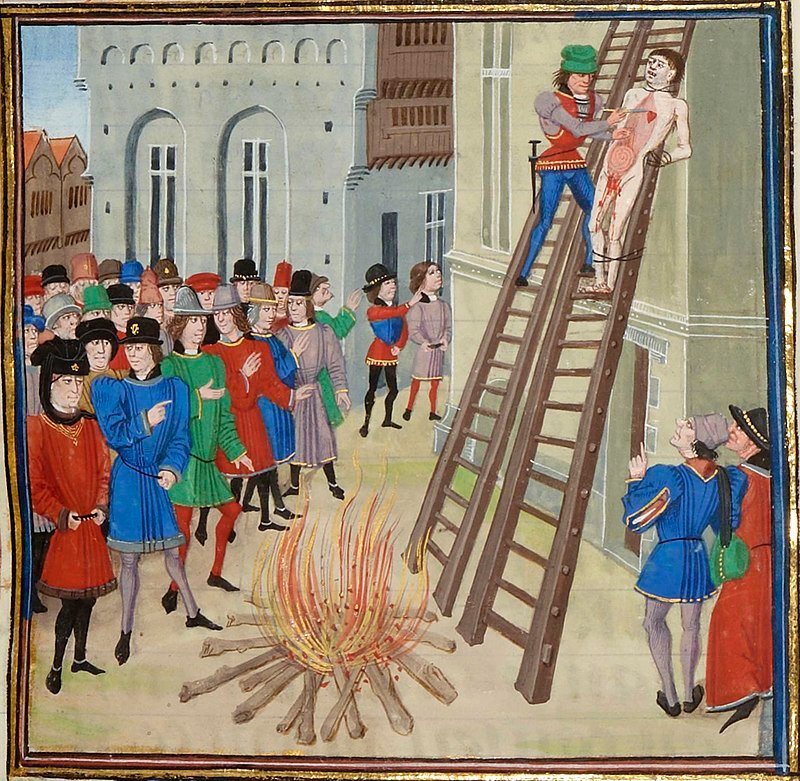
\includegraphics[width=2.67in,height=\textheight]{../figure/hugh.jpg}

}

\caption{\label{fig-hugh}Execution of Hugh Despenser, featuring huge
penis. On 24 November 1326, Hugh Despenser the Younger was gruesomely
executed at Hereford, on the orders of Queen Isabella of France and her
ally, Roger Mortimer. Hugh was hanged, drawn and quartered, and
castrated.}

\end{figure}

\hypertarget{materials-and-methods}{%
\section{Materials and methods}\label{materials-and-methods}}

\hypertarget{data}{%
\subsection{Data}\label{data}}

Penis measurements (and self-reported data) from various sources across
many countries and regions was downloaded from data.world
(https://data.world; last accessed 2023-11-28).

\hypertarget{statistical-analysis}{%
\subsection{Statistical analysis}\label{statistical-analysis}}

We used ggpubr v0.6.0 R package to perform and report statistical tests
\citep{ggpubr}.

\hypertarget{results}{%
\section{Results}\label{results}}

First we analyzed the effect of penis measurement communication to penis
size. We found that self reported penises were slightly bigger
(Fig.~\ref{fig-psize}).

\begin{figure}

{\centering 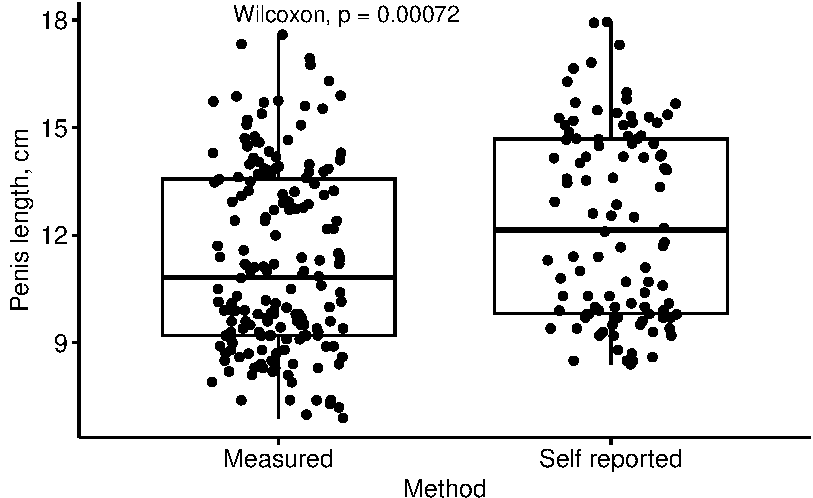
\includegraphics{penis-paper_files/figure-pdf/fig-psize-1.pdf}

}

\caption{\label{fig-psize}Those sneaky bastards self-report bigger
penis.}

\end{figure}

\hypertarget{discussion}{%
\section{Discussion}\label{discussion}}

The perception and reporting of penis size can be influenced by several
factors, and it's important to distinguish between actual physical
measurements and subjective perceptions. Here are some reasons why some
men may report a larger penis size:

\begin{enumerate}
\def\labelenumi{\arabic{enumi}.}
\tightlist
\item
  \textbf{Social and Cultural Influences:}

  \begin{itemize}
  \tightlist
  \item
    Social and cultural factors play a significant role in shaping
    individuals' perceptions of body image, including penis size.
    Societal ideals and media representations may contribute to a desire
    for larger genitalia, leading some individuals to overestimate their
    own size.
  \end{itemize}
\item
  \textbf{Self-Perception Bias:}

  \begin{itemize}
  \tightlist
  \item
    People's self-perception is subjective and can be influenced by
    factors such as self-esteem, body image, and personal experiences.
    Some individuals may perceive their genitals differently than they
    objectively measure.
  \end{itemize}
\item
  \textbf{Measurement Methods:}

  \begin{itemize}
  \tightlist
  \item
    The accuracy of self-reported measurements can vary. Some men may
    measure their penis in a way that provides a larger result, either
    intentionally or due to measurement errors. This could include
    measuring from a different starting point or applying more pressure
    during measurement.
  \end{itemize}
\item
  \textbf{Social Comparison:}

  \begin{itemize}
  \tightlist
  \item
    Individuals may compare themselves to others, and this comparison
    can influence how they perceive their own size. If someone believes
    that a larger size is socially desirable, they may be more likely to
    report a size that aligns with this perceived norm.
  \end{itemize}
\item
  \textbf{Psychological Factors:}

  \begin{itemize}
  \tightlist
  \item
    Psychological factors, such as confidence and self-esteem, can
    influence the way individuals perceive and report their own
    characteristics, including penis size. A person with higher
    self-esteem might be more likely to report a positive self-image.
  \end{itemize}
\item
  \textbf{Pressure to Conform:}

  \begin{itemize}
  \tightlist
  \item
    Societal pressures and expectations related to masculinity and
    sexual performance may contribute to a desire to present oneself in
    a way that aligns with perceived norms. This pressure could
    influence how individuals report their penis size.
  \end{itemize}
\end{enumerate}

It's important to note that there is a wide range of normal variations
in penis size, and there is no standard or ideal size. Scientific
studies have consistently shown that there is considerable diversity in
penis size among men, and factors such as genetics and hormonal
influences contribute to this variation.

In clinical research, accurate measurements are typically obtained by
trained professionals using standardized methods. Self-reported
measurements, on the other hand, may not always reflect objective
reality. Additionally, the emphasis on penis size can sometimes lead to
unrealistic expectations, contributing to body image concerns.

If individuals have concerns about their body image or penis size, it
may be helpful to seek guidance from healthcare professionals or mental
health experts who can provide accurate information and support.

\hypertarget{acknowledgments}{%
\section{Acknowledgments}\label{acknowledgments}}

TP wishes to thank ChatGPT v3.5. TP thanks the members of the members of
the distinguished Wild Animals consortium -- SS, VV, CL, UA.


\nolinenumbers
  \bibliography{bibliography.bib}

\end{document}
